%% LyX 2.4.3 created this file.  For more info, see https://www.lyx.org/.
%% Do not edit unless you really know what you are doing.
\documentclass[english,aspectratio=1610]{beamer}
\usepackage{lmodern}
\renewcommand{\sfdefault}{lmss}
\renewcommand{\ttdefault}{lmtt}
\usepackage[utf8]{inputenc}
\usepackage{babel}
\usepackage{amssymb}
\usepackage{graphicx}
\ifx\hypersetup\undefined
  \AtBeginDocument{%
    \hypersetup{pdfusetitle,
 bookmarks=true,bookmarksnumbered=true,bookmarksopen=false,
 breaklinks=false,pdfborder={0 0 0},pdfborderstyle={},backref=false,colorlinks=false}
  }
\else
  \hypersetup{pdfusetitle,
 bookmarks=true,bookmarksnumbered=true,bookmarksopen=false,
 breaklinks=false,pdfborder={0 0 0},pdfborderstyle={},backref=false,colorlinks=false}
\fi

\makeatletter
%%%%%%%%%%%%%%%%%%%%%%%%%%%%%% Textclass specific LaTeX commands.
% this default might be overridden by plain title style
\newcommand\makebeamertitle{\frame{\maketitle}}%
% (ERT) argument for the TOC
\AtBeginDocument{%
  \let\origtableofcontents=\tableofcontents
  \def\tableofcontents{\@ifnextchar[{\origtableofcontents}{\gobbletableofcontents}}
  \def\gobbletableofcontents#1{\origtableofcontents}
}

%%%%%%%%%%%%%%%%%%%%%%%%%%%%%% User specified LaTeX commands.
\usetheme[progressbar=frametitle]{metropolis}
% or ...

% \setbeamercovered{transparent}
% or whatever (possibly just delete it)
\usepackage{fontspec}
\setsansfont{Fira Sans}
\usepackage{tikz}
\usepackage{amsmath}
\usetikzlibrary{arrows.meta, positioning}
\usetikzlibrary{fit, positioning}

\makeatother

\begin{document}
\title[]{Sovereign Default with Bounded Rationality}
\author[Chen Gao]{Chen Gao}
\institute[PKU]{\inst{1}National School of Development, Peking University\\
}
\date{June 10, 2025}

\makebeamertitle

%\pgfdeclareimage[height=0.5cm]{institution-logo}{institution-logo-filename}
%\logo{\pgfuseimage{institution-logo}}

\AtBeginSubsection[]{%
  \frame<beamer>{ 
    \frametitle{Outline}   
    \tableofcontents[currentsection,currentsubsection] 
  }
}

%\beamerdefaultoverlayspecification{<+->}
\begin{frame}{Outline}
\tableofcontents{}
\end{frame}


\section{Motivation}
\begin{frame}{The Puzzle of Sovereign Spreads}

\textbf{The Empirical Fact: Sovereign Spreads are Puzzling}
\begin{itemize}
\item Emerging market sovereign spreads are \textbf{high} and extremely
\textbf{volatile}.
\item Crises are characterized by sudden \textbf{spikes in spreads}, often
accompanying deep recessions.
\end{itemize}
\begin{figure}
\caption{Argentina’s Default (From (Arellano, 2008))}

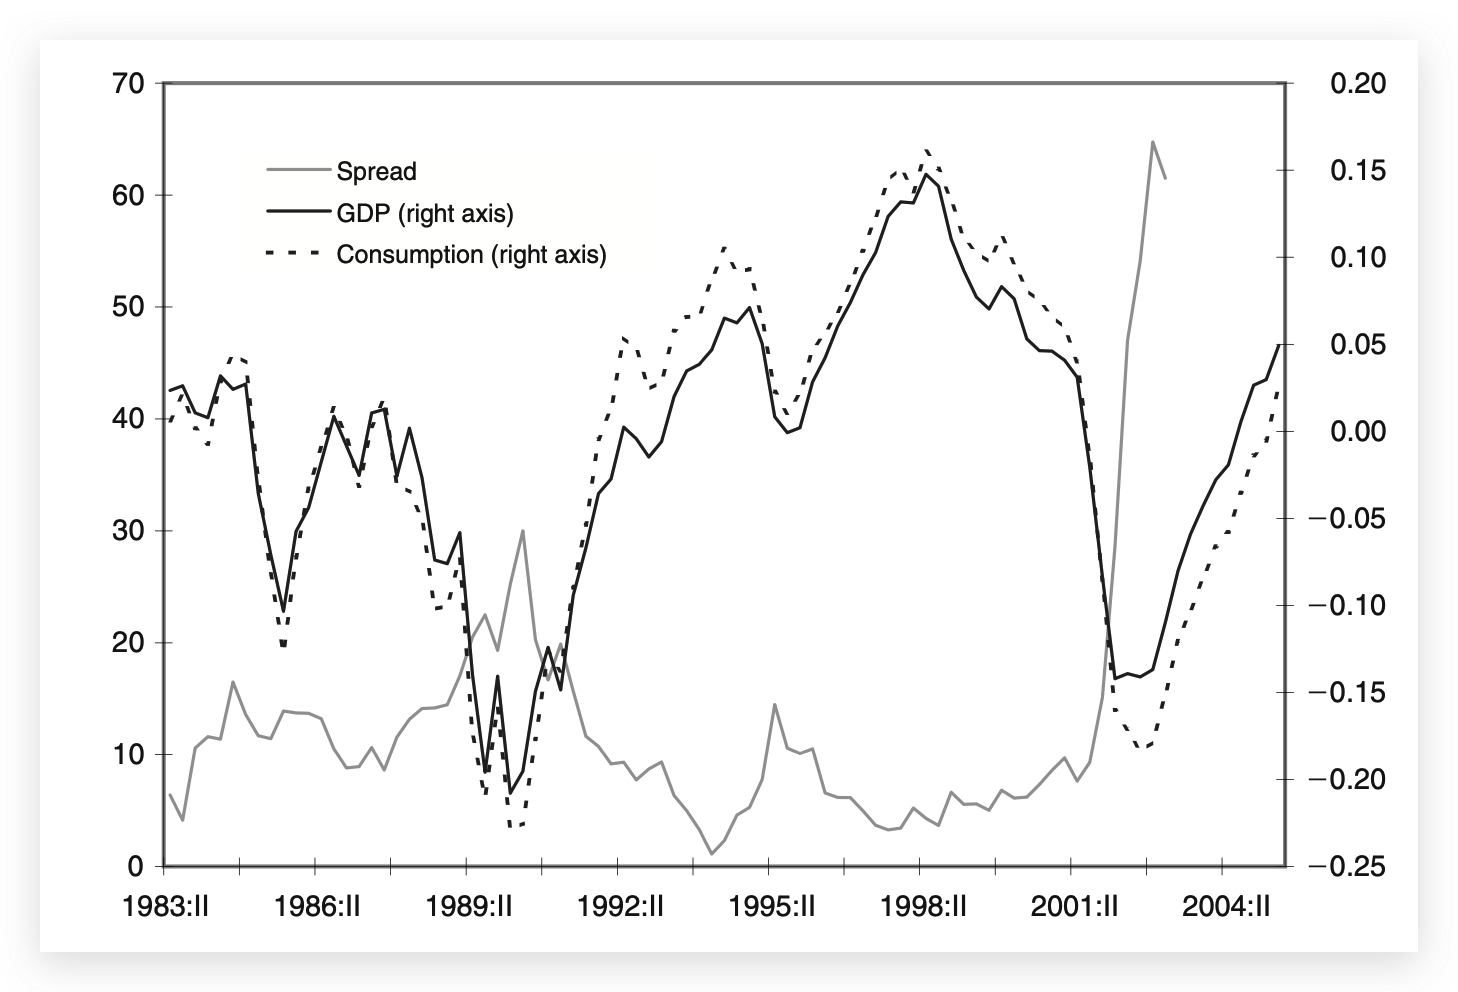
\includegraphics[width=0.5\textwidth]{WorkingProjects/blind/pre/June11_MD_Course/arellanofig1}

\end{figure}
\end{frame}

\end{document}
